\chapter{Survey of Message Broker implementations} 
\label{survey-broker}
In previous chapters we first discussed the traditional messaging broker as it
hosts a queue for simply move data between distributed clients without losing
messages or requiring each component to be always available. Regarding to our
second topic, the streaming of big data we saw that a stream is actually an
abstract version of a message broker with special abilities optimized for
further processing events in real-time. 

In the following survey we want to compare implementations of the most related
broker system by mainly compare the following characteristics---which we already
defined in \todo{ref}---to our reference product Apache Kafka. \todo{ref}

\begin{itemize}
\item Consumption Model 
     \item Delivery Reliability 
         \item Fault Tolerance
\end{itemize}

\section{Implementations}
%\subsection{Traditional Message Broker}

\begin{description}
    \item [Rabbit MQ] \hfill \\
    {
    Performance / Persistence:
    It is possible for persistence to underperform because the persister is
    limited in the number of file handles or async threads it has to work with.
    In both cases this can happen when you have a large number of queues which
    need to access the disk simultaneously. 
    (https://www.rabbitmq.com/persistence-conf.html)

    Several RabbitMQ servers on a local network can be clustered together,
    forming a single logical broker.   In a RabbitMQ Cluster, queues are
    created and live in a single node, and all nodes know about
    all the queues. When a node receives a request to a queue
    that is not available in the current node, it routes the request
    to the node that has the queue.
    To provide high availability
    (HA), RabbitMQ has a mirrored queue arranged in the
    master-slave fashion, and messages are replicated between
    master and slave, so the slave can take over if the master
    has died.
    (http://aidm.googlecode.com/svn/trunk/apache-site/research/papers/mb2.pdf)

    What RabbitMQ clustering doesn't do is provide guarantees against message loss.
    Even if you do everything right (set your messages, queues and exchanges to
    durable, etc.), when a Rabbit cluster node dies, the messages in queues on that
    node can disappear. This is because RabbitMQ doesn't replicate the contents
    of queues throughout the cluster. They live only on the node that owns the
    queue.
    (http://www.cybershovel.com/b/RabbitMQinAction.pdf
    http://pdf.th7.cn/down/files/1312/RabbitMQ%20in%20Action.pdf?yundunkey=1c4e3306d3a07226a40e927b533a8c1841426173782_179979013)
    
    }
    \item [Active MQ] \hfill \\
        {Note: Apache ActiveMQ is an open source message broker written in Java
    together with a full Java Message Service (JMS) client. The Replicated
    LevelDB Store uses Apache ZooKeeper to pick a master from a set of broker
    nodes configured to replicate a LevelDB Store. Then synchronizes all slave
    LevelDB Stores with the master keeps them up to date by replicating all
    updates from the master. ActiveMQ will preserve the order of messages sent
    by a single producer to all consumers on a topic. If there is a single
    consumer on a queue then the order of messages sent by a single producer
    will be preserved as well. Journal: To achieve high performance of durable
    messaging in ACtiveMQ V4.x we strongly recommend you use our high
    performance journal - which is enabled by default. This works rather like a
    database; messages (and transcation commits/rollbacks and message
    acknowledgements) are written to the journal as fast as is humanly possible
    - then at intervals we checkpoint the journal to the long term persistence
    storage (in this case JDBC).Kind of. A message can be loaded directly from the journal if it was swapped out of memory.
    The journal cannot be used, however, to recover a durable subscription as it
    does not keep an ordered index of messages per durable sub. So when a durable
    sub is activated, the journal checkpoints to flush any messages in the journal
    to the long term store and then the long term store is used to recover the
    durable subscription.Brokers cannot share a journal. Each must be
configured with it's own journal. Broker Clustering: The most common mental model of clustering in
a JMS context is that there is a collection of JMS brokers and a JMS client
will connect to one of them; then if the JMS broker goes down, it will
f we just run multiple brokers on a network and tell the clients about them
using either static discovery or dynamic discovery, then clients can easily
failover from one broker to another. However, stand alone brokers don't know
about consumers on other brokers; so if there are no consumers on a certain
broker, messages could just pile up without being consumedauto-reconnect to
another broker. } 

\end{description}


%\subsection{Streaming Broker}
\begin{description}
    \item [Apache Kafka] \hfill \\
        { (What it is) (Creator) (License) (Characteristics according features) Fault-tolerance: Beim conumse kann keine message verloren gehen da log durable, nur bei procuder kann es sein }
    \item [Amazon Kinesis] \hfill \\
    { Amazon Kinesis is a service for real-time processing of streaming big
    data. You can push data from many data producers, rapidly and continuously
as it is generated into Amazon Kinesis, which offers a reliable, highly
scalable service to capture, and store the data. ping that connects all their
distributed systems—DynamoDB, RedShift, S3, etc.—as well as the basis for
distributed stream processing using EC2. \\
 Kinesis keeps messages just for 24 hours no Log Compaction. Thus it cannot be
 used for checkpointing and state store changelogging. Another service must be
 used for durable storage.\\
    
 }
    \item [Scribe] \hfill \\
    { Push based, no pub-sub, static configuration}
    \item [Kastrell] \hfill \\
    {no clustering; no pub-sub}
    \item [Apache Flume] \hfill \\
    {Flume is a distributed service specialized on being a reliable way
    of getting event data into HDFS. The typical deployment consists of a number of
    logical nodes, arranged into three tiers. The first tier is the agent tier.
    Agent nodes are typically installed on the machines that generate the data and
    are the initial point of contact with Flume. They forward data to the
    next tier of collector nodes, which aggregate the separate data flows and
    forward them to the final storage tier. Flume is push based and does not support
    public-subscribe semantics. Therefore Apache Flume can not be used as
    traditional message broker. \cite{apacheflumeDoc}

    \begin{figure}[H]
     \centering
     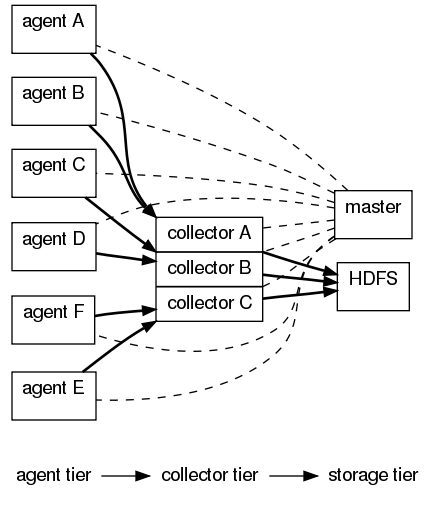
\includegraphics[width=0.4\textwidth]{images/flume-architecture.png}
         \caption{Apache Flume general architecture \cite{apacheflumeDoc}}
        \label{fig:flume-architecture}
    \end{figure}

    }
\end{description}

\begin{landscape}
\section{Conslusion}

\todo[inline]{Welches System passt für welchen Anwendungsfall und welche nicht
(Gründe)}
\end{landscape}

